
\section{Segments and segment computers}

\begin{frame}
  \frametitle{Segments}
 

A segment is a valid and not empty range. 
The concept CSegment is such that: 

  \begin{block}{Types}
\begin{itemize}
  \item Self
  \item ConstIterator
\end{itemize}
  \end{block}

  \begin{block}{Methods}
\begin{itemize}
  \item begin()
  \item end()
\end{itemize}
  \end{block}

\end{frame}

\begin{frame}
  \frametitle{Class of segments}
 
A class of segments can be defined from a valid property P. 
P is valid iff P is true for any range of only one element
and for any not empty range of any segment. 

  \begin{block}{Examples}
\begin{itemize}
  \item - to be a DSS
  \item - to be a balanced word
  \item x to contain at least k elements (k > 1)
\end{itemize}
  \end{block}

\end{frame}

\begin{frame}
  \frametitle{Segment computer}
 
  \begin{block}{Detection problem}
Deciding whether a given segment belongs to a class of segments defined from a valid property P or not. If P is valid, the detection of a segment can be performed in an incremental way: a segment is initialized at a starting element and then can be extended to the neighbors elements if the property P still holds. 
  \end{block}

  \begin{block}{Segment computer}
Segment that can control its own extension (so that the property P remains true)
  \end{block}

 \begin{center}
   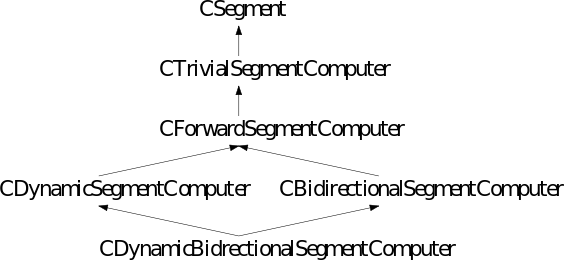
\includegraphics[width=0.6\textwidth]{segmentComputersHierarchy}
 \end{center}

\end{frame}

\begin{frame}[fragile]
  \frametitle{CTrivialSegmentComputer}

Refinement of CSegment that provides in addition the following methods:
\begin{itemize}
 \item void init ( const ConstIterator\& it ) : set the segment to the element pointed to by it.
 \item bool isExtendable () : return 'true' if the segment can be extended to the element pointed to by end() and 'false' otherwise (no extension is performed).
 \item bool extend () : return 'true' and extend the segment to the element pointed to by end() if it is possible, return 'false' and does not extend the segment otherwise.
\end{itemize}

  \begin{block}{Detection of a segment}
\begin{verbatim}

    //s is a segment computer
    //[begin,end) is a range
    s.init( begin );
    while ( (s.end() != end) && (s.extend()) ) {} 

\end{verbatim}
  \end{block}

  \begin{block}{Avoiding infinite loops with circulators}
\begin{verbatim}

    //s is a segment computer
    //c is a circulator
    s.init( c );
    while ( (s.end() != s.begin()) && (s.extend()) ) {}

\end{verbatim}
  \end{block}

\end{frame}

\begin{frame}
  \frametitle{List of segment computers}
 


\begin{itemize}
  \item \alert{ArithmeticalDSS}
  \item ArithmeticalDSS3d
  \item CombinatorialDSS
  \item GeometricalDSS
  \item GeometricalDCA
  \item ThickSegment
  \item ConvexPart
  \item ...
  \item other based on linear programming
\end{itemize}



\end{frame}

\begin{frame}
  \frametitle{Useful functions}
 
The code can be different if an iterator or a circulator is used as the nested ConstIterator type. Moreover, some tasks can be made faster for a given kind of segment computer than for another kind of segment computer. That's why many generic functions are provided in SegmentComputerUtils.h:

\begin{itemize}
 \item maximalExtension, oppositeEndMaximalExtension, maximalSymmetricExtension,
 \item maximalRetraction, oppositeEndMaximalRetraction,
 \item longestSegment (init the segment computer),
 \item firstMaximalSegment, lastMaximalSegment, mostCenteredMaximalSegment,
 \item previousMaximalSegment, nextMaximalSegment,
\end{itemize}



\end{frame}


